
\documentclass[times,singlecolumn]{article}
\usepackage[margin=1in]{geometry}
\usepackage{amsmath}
\usepackage{amsfonts}
\usepackage{graphicx}
\usepackage{xcolor}
\usepackage{ulem}
\usepackage{hyperref}
\input{sym}

\newcommand{\ubfu}{\underline{\bfu}}
\newcommand{\ubfx}{\underline{\bfx}}

\newtheorem{prob}{Problem}


\title{ECE 417/598: What can you find from two images}
\author{Instructor: Vikas Dhiman}
\DeclareMathOperator{\diag}{diag}
\begin{document}
\maketitle
\begin{tabular}{p{0.5\linewidth}p{0.5\linewidth}}
  (1) Student name:& Student email: \\
\end{tabular}

\paragraph{Things to recall}
\begin{enumerate}
  \item Projection of a 3D point to an image $\lambda \bfu = K \bfX$.
  \item Transformation of coordinates $\bfX' = R \bfX + \bft$.
  \item A 2D line passing through two points $\bfu_1 \in \bbP^2$ and $\bfu_2 \in
    \bbP^2$ is given by cross product $\bfl = \bfu_1 \times \bfu_2$.
  \item A cross product can be represented as a matrix vector product,
    \[
      \bfu_1 \times \bfu_2 = \begin{bmatrix}
                               0 & -x_1 & y_1\\
                               x_1 & 0  & -w_1\\
                               -y_1 & w_1  & 0
                               \end{bmatrix} \bfu_2
      \], where $\bfu_1 = [x_1, y_1, w_1]^\top$.
   \item Cross product magnitude is given by $ \| \bfu_1 \times \bfu_2 \| =
     \|\bfu_1 \| \|\bfu_2 \| \sin(\theta)$ where $\theta$ s the angle between
     $\bfu_1$ and $\bfu_2$.
\end{enumerate}

\begin{prob}
  When the depth corresponding to the point $\bfu$ in the left image is unknown,
  the possible
  pixels ($\bfu'$) on the right image that can correspond to  the point form a
  line $\bfl'$. Let the intrinsic camera matrix of left camera be $K$, that of
  right camera be $K'$. Let the rotation and translation of the camera
coordinates from the left camera to the right camera be $R$ and $\bft$
respectively. Find the line $\bfl'$  in terms of other given quantities.
  \\
  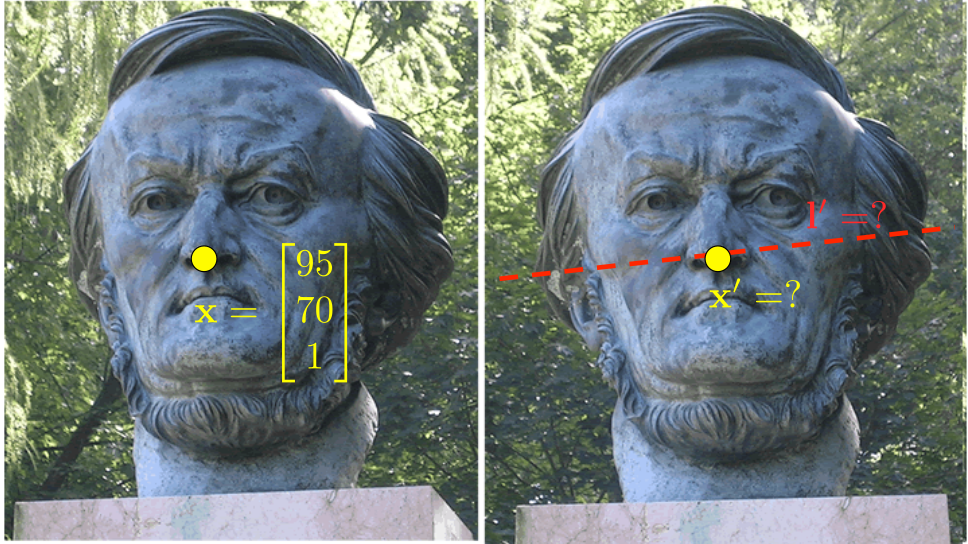
\includegraphics[width=0.5\linewidth]{media/stereo-images.png.pdf}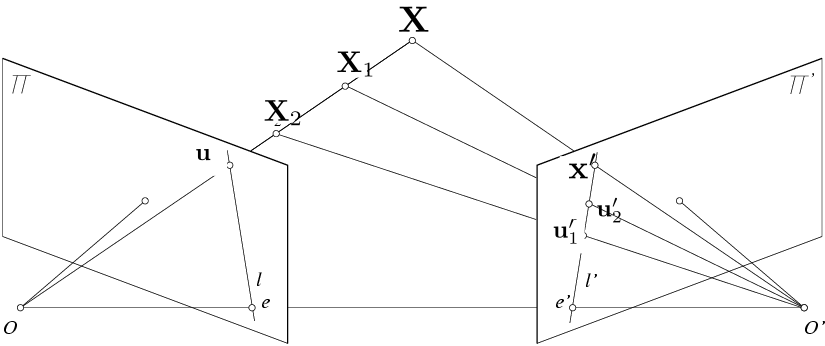
\includegraphics[width=0.5\linewidth]{media/epipolar-constraint.png.pdf}
\end{prob}

\begin{enumerate}
\item Find the equation of ray corresponding to the pothole in the left image.
  In other words, write the equation of the ray corresponding to the point
  $\bfu$, in the first camera frame.
  \\
  \[ \bfX = \lambda K^{-1} \bfu \]

\item Assume the rotation matrix $R$ and translation vector $\bft$, so
  that they transform any point in the left coordinate frame to a point in the
  right coordinate frame. ($\bfX' = R \bfX+ \bft$). Transform the equation of
  ray from the left coordinate frame to the right coordinate frame.
  \\
  \[ \bfX' = R \bfX + \bft \]

\item Project the 3D point $\bfX'$ on the  right camera, call it $\bfu'$.
  \\
  \[ \bfu' = \lambda' K'\bfX' = \lambda' K' (R \bfX + \bft) = \lambda' K'
    (R(\lambda K^{-1} \bfu)  + \bft) = \lambda' \lambda K' R K^{-1} \bfu +
    \lambda' K' \bft \]


\item The point on right image $\bfe'$ is the projection of origin $(0, 0)$ of left
  camera. Find $\bfe'$ (also called the 
  \[
    \bfe' = \lambda'_e K' R \begin{bmatrix} 0 \\ 0 \\ 0\end{bmatrix} +
    \lambda'_e K' \bft = \lambda'_e K' \bft
    \]

\item Find a line $\bfl'$ that passes through both $\bfu'$ and $\bfe'$, such
  that $\bfl'^\top \bfu' = 0$ and $\bfl'^\top \bfe' = 0$.
  \[
    \bfl' = \bfe' \times \bfu'  = \lambda'_e K' \bft \times 
    (\lambda' \lambda K' R K^{-1} \bfu +
    \lambda' K' \bft)
    = \lambda'_e K' \bft \times 
    \lambda' \lambda K' R K^{-1} \bfu + \underbrace{\lambda'_e K' \bft \times
      \lambda' K' \bft}_{ = \mathbf{0}_{3\times 1}}
    \]

    \[ \bfl' = K' \bft \times K' R K^{-1}\bfu\] 

  \item Define Fundamental matrix $F$ such that $\bfu^{'\top} F\bfu = 0$. What is
    Fundmental matrix in terms of $K, K', R$ and $t$.
    \[ \bfu^{'\top} \bfl' = 0\]
    \[ \bfu^{'\top} (K' \bft \times K' R K^{-1}\bfu)  = 0\]
    \[ \bfu^{'\top} ([K' \bft]_{\times} K' R K^{-1}\bfu)  = 0\]
    \[ \bfu^{'\top} \underbrace{[K' \bft]_{\times} K' R K^{-1} }_{F} \bfu  = 0\]

   \item Define normalized coordinates as $\bfp = K^{-1}\bfu$ and $\bfp' =
     K'^{-1} \bfu'$.  Repeat the above process for $\bfp$ and $\bfp'$.
     \\
     \[  \bfp' =  R \bfp + \bft \]
     \[  \bfe'_p =  \bft \]
     Normal of the plane that contains both $\bfp$ and $\bfe'_p$,
     \[ \bfn' = \bfe'_p \times \bfp'  = \bft \times (R \bfp + \bft) = \bft
       \times R\bfp \]
     Equation of the plane with normal $\bfn'$,
     \[ \bfp^{'\top} \bfn  = 0\]
     \[ \bfp^{'\top} [ \bft]_{\times} R   \bfp  = 0\]

  \item Define Essential matrix $E$ such that $\bfp^{'\top} E\bfp = 0$. What is
    Essential matrix in terms of $ R$ and $t$?
    \[ \bfp^{'\top} \underbrace{[ \bft]_{\times} R}_{E}   \bfp  = 0\]

  \item Find a relationship between Fundamental matrix and Essential matrix.
    \[ \bfp^{'\top} E \bfp  = 0 \]
    \[ \bfu^{'\top} \underbrace{K^{'-\top} E K^{-1}}_{F} \bfu  = 0 \]
    \[ F = K^{'-\top} E K^{-1} \]
    \[ K^{'\top} F K = E \]
\end{enumerate}

\paragraph{Matching}
\includegraphics[width=0.5\linewidth]{media/stereo-images-matching.pdf}
\vspace{10em}

\begin{prob}
  Let $n \ge 8$ pairs of correspondence points be given between left image and
  the right images as $\bfu_1, \bfu_2, \dots, \bfu_n$ and $\bfu'_1, \bfu'_2,
  \dots, \bfu'_n$ respectively. Let the left and right camera matrices be given
  as $K$ and $K'$ respectively. Find the fundamental and essential matrix.
  \\
  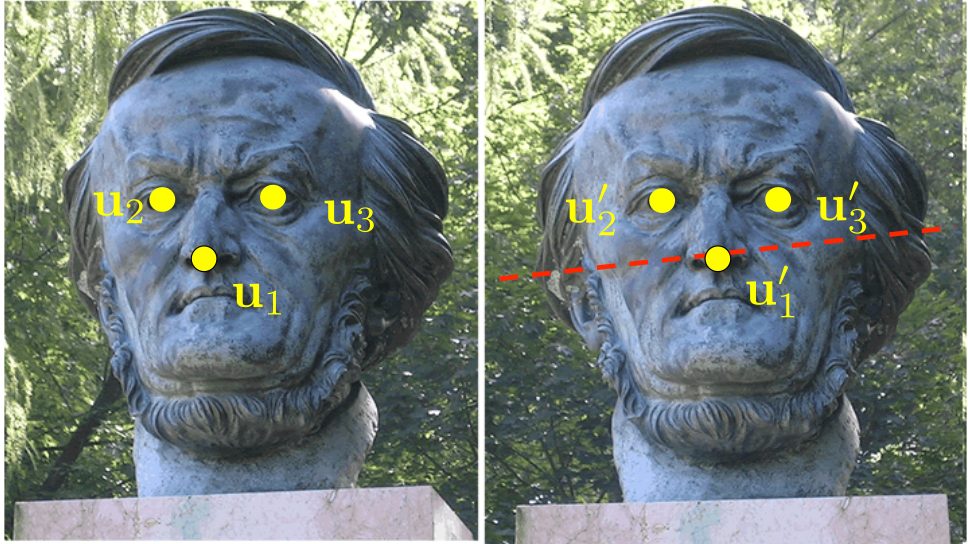
\includegraphics[width=0.5\linewidth]{media/stereo-images-correspond.pdf}
\end{prob}

\begin{enumerate}
  \item Convert equations $\bfu_i^{'\top} F \bfu_i = 0$ for all $i \in \{1, \dots,
    n\}$ into $A\bfy = 0$ form to find the unknown matrix $F$.
    \vspace{10em}
  \item Write $F = \begin{bmatrix} \bff_1^\top \\ \bff_2^\top \\ \bff_3^\top\end{bmatrix}$ in terms of its rows.
    \vspace{10em}

  \item Expand $\bfu_i^{'\top} F\bfu_i = 0$  in terms of the rows of $F$.
    \vspace{10em}
  \item Rearrange terms so that we can get the unknowns on the right hand side,
    so that we have an equation in the form $A_i \bfy = 0$ for a single point.
    \vspace{10em}
  \item Concatenate equations from multiple points to a big matrix and equation
    of the form $A \bfy = 0$.
    \vspace{10em}
  \item Solve the above equation using Singular value decomposition.
    \vspace{10em}
  \item Find essential matrix from Fundamental matrix
    \vspace{10em}

\end{enumerate}

\begin{prob}
  (Optional) Find the Rotation $R$ and translation $\bft$ from the Essential matrix $E =
  \bft \times R$.
\end{prob}
\paragraph{Solution}
\begin{enumerate}
  
\item \[ Z = \begin{bmatrix} 0 & 1 & 0 \\ -1 & 0 & 0 \\ 0 & 0 & 0\end{bmatrix} \]
\item \[ W = \begin{bmatrix} 0 & -1 & 0 \\ 1 & 0 & 0 \\ 0 & 0 & 1\end{bmatrix}
    = \diag(1, 1, 0) Z \]
\item Let the SVD of $E$ be \[ E = U\Sigma V^\top \]
\item \[ E = \underbrace{(UZU^\top)}_{[\bft]_\times} \underbrace{(UW^\top V^\top)}_{R}  \]
\end{enumerate}


\paragraph{Things to take away}
\begin{enumerate}
  \item Epipolar line can be found by projecting two points from left camera to
    the right camera. One of the points can be origin.
  \item Definition of Fundamental matrix and Essenstial matrix.
  \item How to find essential matrix from given correspondence points?
  \item How to find Rotation and translation from essential matrix?
\end{enumerate}


\end{document}